%\documentclass{buthesis}         %Default is author-year citation style
\documentclass[numbib]{buthesis}  %Gives numerical citation style
%\documentclass[twoadv}{buthesis} %Allows entry of second advisor
\usepackage{graphics}             %Select graphics package
%\usepackage{graphicx}            %
\usepackage{amsthm}               %Add other packages as necessary
\begin{document}
\butitle{This is the title of my thesis.  It will come out in capital
letters as requested}
\author{A. Student}
\degree{Bachelor of Science}
\department{Physics \& Astronomy}
\advisor{Martin K. Ligare}
%\advisorb{Jane Doe}              %Second advisor if necessary
\chair{David Schoepf}
\maketitle
\frontmatter

\acknowledgments{Thanks to everybody I know, from my parents, to my 
childhood friends and kindergarten teacher.  I didn't learn everything
I needed to know in kindergarten, but it came close.  I guess
I should thank my thesis advisor too.}

\tableofcontents

\listoftables

\listoffigures

\abstract{Here is my abstract. Here is my abstract. Here is my abstract. 
Here is my abstract. Here is my abstract. Here is my abstract. Here is my
abstract. Here is my abstract.}

\mainmatter

\chapter{Introduction}
This paragraph will be written with standard margins. I will repeat
lines as necessary to make it long enough. This paragraph has a 
citation \citep{SMI04} that you can see.
I will repeat lines as necessary to
make it long enough. This paragraph will be written with standard
margins. I will repeat lines as necessary to make it long enough.

This paragraph will be written with standard margins. I will repeat
lines as necessary to make it long enough. This paragraph 
will be written with standard margins. I will repeat lines as necessary to
make it long enough. This paragraph will be written with standard
margins. I will repeat lines as necessary to make it long enough.

\chapter[Long chapter]{This chapter has a long name.}
This paragraph will be written with standard margins. I will repeat
lines as necessary to make it long enough. This paragraph will be
written with standard margins. I will repeat lines as necessary to
make it long enough. This paragraph will be written with standard
margins. I will repeat lines as necessary to make it long enough.

This paragraph will be written with standard margins. I will repeat
lines as necessary to make it long enough. This paragraph will be
written with standard margins. I will repeat lines as necessary to
make it long enough. This paragraph will be written with standard
margins. I will repeat lines as necessary to make it long enough.
This paragraph will be written with standard margins. I will repeat
lines as necessary to make it long enough. This paragraph will be
written with standard margins. I will repeat lines as necessary to
make it long enough. This paragraph will be written with standard
margins. I will repeat lines as necessary to make it long enough.

This paragraph will be written with standard margins. I will repeat
lines as necessary to make it long enough. This paragraph will be
written with standard margins. I will repeat lines as necessary to
make it long enough. This paragraph will be written with standard
margins. I will repeat lines as necessary to make it long enough. This
paragraph will be written with standard margins. I will repeat lines
as necessary to make it long enough. This paragraph will be written
with standard margins. I will repeat lines as necessary to make it
long enough. This paragraph will be written with standard margins. I
will repeat lines as necessary to make it long enough.

Where does this go?

This is the equation of a straight line:
\begin{equation}
y = mx + b.
\end{equation}
This paragraph will be written with standard margins. I will repeat
lines as necessary to make it long enough. This paragraph will be
written with standard margins. I will repeat lines as necessary to
make it long enough. This paragraph will be written with standard
margins. I will repeat lines as necessary to make it long enough.


This paragraph will be written with standard margins. I will repeat
lines as necessary to make it long enough. This paragraph will be
written with standard margins. I will repeat lines as necessary to
make it long enough. This paragraph will be written with standard
margins. I will repeat lines as necessary to make it long enough.
This paragraph will be written with standard margins. I will repeat
lines as necessary to make it long enough. This paragraph will be
written with standard margins. I will repeat lines as necessary to
make it long enough. This paragraph will be written with standard
margins. I will repeat lines as necessary to make it long enough.


This paragraph will be written with standard margins. I will repeat
lines as necessary to make it long enough. This paragraph will be
written with standard margins. I will repeat lines as necessary to
make it long enough. This paragraph will be written with standard
margins. I will repeat lines as necessary to make it long enough. This
paragraph will be written with standard margins. I will repeat lines
as necessary to make it long enough. This paragraph will be written
with standard margins. I will repeat lines as necessary to make it
long enough. This paragraph will be written with standard margins. I
will repeat lines as necessary to make it long enough.

Where does this go?

This is the equation of a straight line:
\begin{equation}
y = mx + b.
\end{equation}
This paragraph will be written with standard margins. I will repeat
lines as necessary to make it long enough. This paragraph will be
written with standard margins. I will repeat lines as necessary to
make it long enough. This paragraph will be written with standard
margins. I will repeat lines as necessary to make it long enough.


This paragraph will be written with standard margins. I will repeat
lines as necessary to make it long enough. This paragraph will be
written with standard margins. I will repeat lines as necessary to
make it long enough. This paragraph will be written with standard
margins. I will repeat lines as necessary to make it long enough.
This paragraph will be written with standard margins. I will repeat
lines as necessary to make it long enough. This paragraph will be
written with standard margins. I will repeat lines as necessary to
make it long enough. This paragraph will be written with standard
margins. I will repeat lines as necessary to make it long enough.


This paragraph will be written with standard margins. I will repeat
lines as necessary to make it long enough. This paragraph will be
written with standard margins. I will repeat lines as necessary to
make it long enough. This paragraph will be written with standard
margins. I will repeat lines as necessary to make it long enough. This
paragraph will be written with standard margins. I will repeat lines
as necessary to make it long enough. This paragraph will be written
with standard margins. I will repeat lines as necessary to make it
long enough. This paragraph will be written with standard margins. I
will repeat lines as necessary to make it long enough.

Where does this go?

This is the equation of a straight line:
\begin{equation}
y = mx + b.
\end{equation}
This paragraph will be written with standard margins. I will repeat
lines as necessary to make it long enough. This paragraph will be
written with standard margins. I will repeat lines as necessary to
make it long enough. This paragraph will be written with standard
margins. I will repeat lines as necessary to make it long enough.
This paragraph will be written with standard margins. I will repeat
lines as necessary to make it long enough. This paragraph will be
written with standard margins. I will repeat lines as necessary to
make it long enough. This paragraph will be written with standard
margins. I will repeat lines as necessary to make it long enough.

\begin{figure}[t]
\begin{center}
\scalebox{0.75}{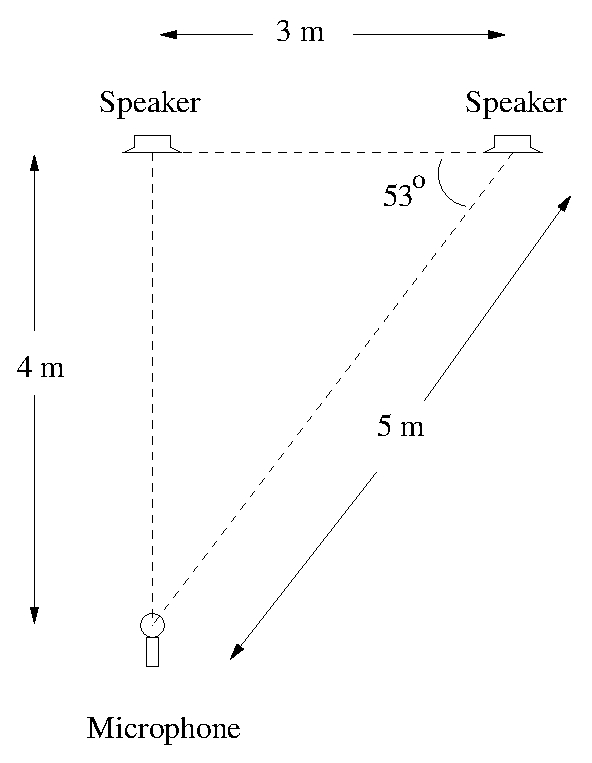
\includegraphics{speaker.eps}}
\end{center}
\caption[Short caption for figure]{This is a figure from PHYS 212 exam 2.  I
want to see the font used for the caption, and width of lines, etc. I
may want to design our own figure environment.  Figures not
automatically centered either.}
\label{f_speaker}
\end{figure}

This paragraph will be written with standard margins. I will repeat
lines as necessary to make it long enough. This paragraph will be
written with standard margins. I will repeat lines as necessary to
make it long enough. This paragraph will be written with standard
margins. I will repeat lines as necessary to make it long enough.
This paragraph will be written with standard margins. I will repeat
lines as necessary to make it long enough. This paragraph will be
written with standard margins. I will repeat lines as necessary to
make it long enough. This paragraph will be written with standard
margins. I will repeat lines as necessary to make it long enough.


This paragraph will be written with standard margins. I will repeat
lines as necessary to make it long enough. Here's a citation \citep{LIG05}.
This paragraph will be
written with standard margins. I will repeat lines as necessary to
make it long enough. This paragraph will be written with standard
margins. I will repeat lines as necessary to make it long enough. This
paragraph will be written with standard margins. I will repeat lines
as necessary to make it long enough. This paragraph will be written
with standard margins. I will repeat lines as necessary to make it
long enough. This paragraph will be written with standard margins. I
will repeat lines as necessary to make it long enough.

Where does this go?

This is the equation of a straight line:
\begin{equation}
y = mx + b.
\end{equation}

\backmatter

%%%%Use following line if bibtex is being used.
%\bibliography{samplebib.bib}


%%%Use following if references are being entered by hand.
\begin{thebibliography}{99}
\bibitem[Smith(2004)]{SMI04}J.~Smith, ``A very good paper paper,''  
J.~Good Phys., {\bf 2}, 294 (2004).
\bibitem[Ligare(2005)]{LIG05}M.~Ligare, ``An even better paper,''
J.~Better Phys., {\bf 2}, 294 (2005).
\end{thebibliography}

\end{document}
